\documentclass{ieeeojies}
\usepackage{cite}
\usepackage{amsmath,amssymb,amsfonts}
\usepackage{algorithm}
\usepackage{algpseudocode}
\usepackage{graphicx}
\usepackage{textcomp}
\usepackage{array}
\usepackage[table]{xcolor}
\usepackage{multirow}
\usepackage{multicol}
\usepackage{float}
\usepackage[hidelinks]{hyperref}


\def\BibTeX{{\rm B\kern-.05em{\sc i\kern-.025em b}\kern-.08em
    T\kern-.1667em\lower.7ex\hbox{E}\kern-.125emX}}

\begin{document}
\title{USING DEEP LEARNING MODELS WITH OPTIMIZATION ALGORITHM AND STATISTICAL MODELS TO FORECAST THE STOCK PRICE OF THREE VIETNAMESE BANKS}

\author{\uppercase{Ngo van manh}\authorrefmark{1},
\uppercase{Nguyen ngoc thanh\authorrefmark{2}, and Tran Quoc khang}\authorrefmark{3}}

\address[1]{Faculty of Information Systems, University of Information Technology, (e-mail: 21522328@gm.uit.edu.vn)}
\address[2]{Faculty of Information Systems, University of Information Technology, (e-mail: 21522600@gm.uit.edu.vn)}
\address[3]{Faculty of Information Systems, University of Information Technology, (e-mail: 21522200@gm.uit.edu.vn)}

\markboth
{Author \headeretal: Author 1, Author 2, Author 3}
{Author \headeretal: Author 1, Author 2, Author 3}

\begin{abstract}
This paper conducts an analysis and stock price forecasts for VCB, BID, and CTG, the top three banks in Vietnam, crucial entities in the financial sector. These banks play a pivotal role in the country's economic landscape. Leveraging a diverse set of models including Linear Regression, ARIMA, RNN, GRU, LSTM, and MLP, we predict the close stock prices of these banks. Furthermore, we employ optimization algorithms such as Nadam and Adadelta to enhance the performance of our Deep learning model and compare when not using optimization models to give insights on efficiency. By scrutinizing stock price fluctuations and employing advanced forecasting methodologies, this study provides valuable insights for investors and stakeholders in the Vietnamese banking industry.
\end{abstract}

\begin{keywords}
Stock price forecasting, Vietnamese banks, VCB, BID, CTG, Linear Regression, ARIMA, RNN, GRU, LSTM, MLP, Nadam, Adadelta.
\end{keywords}

\titlepgskip=-15pt

\maketitle

\section{Introduction}
The stock market refers to the collection of markets and ex-change centers where economic activities like buying, selling,and deploying shares of publicly held companies take place.Such financial practices are conducted through institutionalized formal exchanges through over‐the‐counter marketplaces that function under a defined set of regulations. The stock market is a very dynamic and uncertain field, so the stock market prediction naturally becomes a burning topic. Due to the advancement of computational power in recent times, pre-dicting the stock market has been much faster and accurate.Artificial Intelligence and machine learning models play a crucial role in predicting stock prices and, hence, deter-mining an accurate result \cite{b1} \\
This study chooses the Ho Chi Minh Stock Exchange (HOSE) in VietNam, including three different stock market of three VietNamese Banks. There are many algorithms and techniques that help us predict prices. In this paper, we will use Linear Regression, LSTM, RNN, GRU, MLP models to predict the stock prices of VietcomBank, BIDV, VietinBank for the next 30 days

\section{Related Works}
This section reviews relevant studies that explore the application of mathematical models for stock price prediction. In this study, we evaluate the performance of six algorithms: Linear regression, ARIMA, RNN, GRU, LSTM, and MLP (using Nadam and Adadelta optimizers) for forecasting stock prices in Vietnam. 

A Multi Parameter Forecasting for Stock Time Series Data Using LSTM and Deep Learning Model by Shahzad Zaheer et al. introduces a method using LSTM and deep learning to predict stock prices, focusing on predicting both closing and high prices for the next day. Their approach outperforms existing methods in accuracy for short-term forecasting. \cite{b2} 

A Comparative Research of Stock Price Prediction of Selected Stock Indexes and the Stock Market by Using ARIMA Model by Nayab Minhaj et al. demonstrates the effectiveness of the ARIMA model in predicting Johnson \& Johnson (JNJ) stock prices in the short term, showing superiority over traditional methods. \cite{b3} 

Nadam: A novel long term solar photovoltaic power forecasting approach using LSTM with Nadam optimizer by Jatin Sharma et al. compares LSTM models using various optimizers and shows that the Nadam optimizer significantly enhances forecasting accuracy compared to other methods. \cite{b4} 

ADADELTA: An Adaptive Learning Rate Method by Matthew D. Zeiler introduces Adadelta, a robust per-dimension learning rate method that adapts dynamically during training, demonstrating effectiveness across different datasets and architectures. \cite{b5} 

Stock Price Prediction Using Deep Learning Techniques by Lee J. et al. explores various deep learning models, including MLP, for stock price prediction. The study highlights the effectiveness of MLP models, particularly when using advanced optimizers like Nadam and Adadelta, in capturing complex patterns in stock data and achieving high prediction accuracy. \cite{b6}

The aforementioned studies provide a foundation for understanding the strengths and weaknesses of different models and optimizers in stock price prediction. In our research, we aim to build on these insights by comparing the performance of Linear regression, ARIMA, RNN, GRU, LSTM, and MLP models using Nadam and Adadelta optimizers, specifically in the context of the Vietnamese stock market.

\section{Materials and Methodology}
\subsection{Dataset}
The historical stock price of Joint Stock Commercial Bank for Foreign Trade of Vietnam (VCB), Bank for Investment and Development of Vietnam (BIDV) and Military Commercial Joint Stock Bank (CTG) from 01/01/2015 to 01/06/2024 will be applied. The data contains column such as Date, Price, Open, High, Low, Close, Adj Close, Volume. As the goal is to forecast high and low prices, data relating to column “High", "Low" (VND) will be processed.

\subsection{Descriptive Statistics}
\begin{table}[H]
  \centering
  \renewcommand{\arraystretch}{1.1}
  \caption{VCB, BIDV, CTG’s Close Price Descriptive Statistics}
    \begin{tabular}{|>{\columncolor{red!20}}c|c|c|c|}
        \hline
         \rowcolor{red!20} 
            Close & VCB & BID & CTG \\ \hline
            Count & 2339 & 2345 & 2345 \\ 
            Mean & 49573.072 & 25785.842 & 19510.972 \\
            Std & 22421.328 & 10557.657 & 7060.096 \\ 
            Min & 15680.371 & 9101.713 & 9637.772 \\ 
            25\% & 25332.525 & 15240.078 & 13451.279 \\ 
            50\% & 50432.793 & 26740.693 & 16606.089 \\ 
            75\% & 66027.141 & 32138.221 & 25729.027 \\ 
            Max & 97400 & 54400 & 37719.051\\ \hline
    \end{tabular}
\end{table}

\begin{figure}[H]
    \centering
    \begin{minipage}{0.45\textwidth}
    \centering
    \includegraphics[width=1\textwidth]{bibliography/DataOverView/vcb.png}
    \caption{Vietcombank stock close price's line chart}
    \label{fig:1}
    \end{minipage}
\end{figure}

\begin{figure}[H]
    \centering
    \begin{minipage}{0.45\textwidth}
    \centering
    \includegraphics[width=1\textwidth]{bibliography/DataOverView/bid.png}
    \caption{BIDV stock close price's line chart}
    \label{fig:1}
    \end{minipage}
    
\end{figure}\begin{figure}[H]
    \centering
    \begin{minipage}{0.45\textwidth}
    \centering
    \includegraphics[width=1\textwidth]{bibliography/DataOverView/ctg.png}
    \caption{Vietinbank stock close price's line chart}
    \label{fig:1}
    \end{minipage}
\end{figure}

\section{Methodology}
\subsection{Linear Regression} 
Regression models are used for describing relationships between variables by fitting a line to the observed data. Regression can estimate how a dependent variable changes as the independent variables change. Multiple linear regression is used for estimating the relationship between two or more independent variables and one dependent variable 
A multiple linear regression model has the form: \cite{b7}
\[Y=\beta_0+\beta_1X_1+\beta_2X_2+\cdots+\beta_kX_k+\varepsilon\]
Where:\\
	\indent\textbullet\ Y is the predicted value of the dependent variable.\\
	\indent\textbullet\ \(X_1, X_2, \ldots, X_k\) are the independent variables.\\
	\indent\textbullet\ \(\beta_0\) is the intercept term.\\
	\indent\textbullet\ \(\beta_1,..., \beta_k\) are the regression coefficients for the independent variables.\\
	\indent\textbullet\ \(\varepsilon\) is the error term.    

 \subsection{ARIMA} 
An autoregressive integrated moving average (ARIMA) model is a statistical tool utilized for analyzing time series data, aimed at gaining deeper insights into the dataset or forecasting forthcoming trends. \cite{b8}
\\
\textit{\textbf{Autoregressive (AR)}}
\\
AR is Auto Regression, and p is the number of autoregressive terms . The equation for AR model is: 
\[
Y_t = \varphi_1Y_{t-1} + \varphi_2Y_{t-2} + ... + \varphi_pY_{t-p} + \delta + \varepsilon_t
\]
\textit{\textbf{Moving Average (MA)}}
\\
MA is the Moving Average, and q is the number of terms in the moving average. The equation for MA model is:  
\[
Y_t = \theta_1\varepsilon_{t-1} + \theta_2\varepsilon_{t-2} + ... + \theta_p\varepsilon_{t-p} + \mu + \varepsilon_t  
\]
\textit{\textbf{Differencing (I) }}
\\
Last, the I part is Integrated, and d is the number of differences (order) required to make it a stationary sequence. For example:
\begin{align*}
    d=0: & \quad \Delta Y_t = Y_t \\
    d=1: & \quad \Delta Y_t = Y_t - Y_{t-1} \\
    d=2: & \quad \Delta Y_t = \left(Y_t - Y_{t-1}\right) - \left(Y_{t-1} - Y_{t-2}\right)
\end{align*}5

After combining them, we will have the ARIMA (p, d, q) express as follow:
\begin{align*}
\Delta Y_t = \mu + \varphi_1 Y_{t-1} + \varphi_2 Y_{t-2} + \cdots + \varphi_p Y_{t-p} \\
+ \theta_1 \varepsilon_{t-1} + \theta_2 \varepsilon_{t-2} + \cdots + \theta_p \varepsilon_{t-p} + \varepsilon_t
\end{align*}

\subsection{GRU}
GRU is another version of the RNN algorithm that solves the problems of vanishing and exploding gradients in traditional RNN when learning long-term dependencies. GRU consists of three main components (Reset gate, Update gate and Output).Those gates enable the GRU to update and choose selectively
information from previous time steps, allowing it to capture long-term dependencies in sequences \cite{b9}
\begin{figure}[H]
    \centering
    \begin{minipage}{0.45\textwidth}
    \centering
    \includegraphics[width=0.8\textwidth]{bibliography/GRU.svg.png}    
    \label{fig:1}
    \caption{GRU unit's structure}
    \end{minipage}
\end{figure}
\begin{itemize}
    \item Reset gate is used to decide what information from the past should be forgotten by using a sigmoid function.\\
        \[r_t = \sigma(W_r [h_{t-1}, x_t] + b_r) \]
    
    \item Update gate just like a combination of forget gate and input gate in LSTM, it combined with the current input at a specific timestep to decide how much information from the previous state will be retained and how much new information will be added.\\
        \[ z_t = \sigma(W_z [h_{t-1}, x_t] + b_z) \]
    \item The output using the current memory state  and is typically followed by an activation function.\\
        \[ \tilde{h}_t = \tanh(W_h [r_t h_{t-1}, x_t]) \]
        \[ h_t = (1 - z_t) h_{t-1} + z_t \tilde{h}_t \]
\end{itemize}

\subsection{RNN} 
RNN is called recurrent neural network because the current output of a sequence is also related to the previous output. The network will memorize  the  previous  information and apply  it  to  the calculation of  the  current  output and the input of the hidden layer not only  includes the output of  the input layer It also  includes  the output of the  hidden layer at the previous moment. RNN can process sequence data of any length. \\
The basic structure of an RNN involves a recurrent layer where sequential inputs are processed at each time step. At each time step \(t\), the RNN receives the input \(x_t\) and the hidden state from the previous time step \(h_{t-1}\), then calculates the current hidden state \(h_t\) and the output \(\hat{y}_t\). \cite{b10}
\[
h_t = \phi(W_{xh} x_t + W_{hh} h_{t-1} + b_h)
\]
\[
\hat{y}_t = \sigma(W_{hy} h_t + b_y)
\]
Where:
\begin{itemize}
    \item \(x_t\): Input at time step \(t\)
    \item \(h_t\): Hidden state at time step \(t\)
    \item \(\hat{y}_t\): Output at time step \(t\)
    \item \(W_{xh}\): Weight matrix for input to hidden state
    \item \(W_{hh}\): Weight matrix for hidden state to hidden state
    \item \(W_{hy}\): Weight matrix for hidden state to output
    \item \(b_h, b_y\): Bias terms
    \item \(\phi\): Activation function (typically tanh or ReLU)
    \item \(\sigma\): Output activation function (typically softmax or sigmoid)
\end{itemize}
\begin{figure}[H]
    \centering
    \begin{minipage}{0.45\textwidth}
    \centering
    \includegraphics[width=0.8\textwidth]{bibliography/RNN/model_struct.png}    
    \label{fig:1}
    \caption{RNN model's network \cite{b11}}
    \end{minipage}
\end{figure}
\subsection{LSTM} 
Long Short-Term Memory (LSTM) networks are a specialized type of recurrent neural network (RNN) designed to address the issue of learning from long sequences of data. LSTMs achieve this through memory cells and gates, which regulate information flow, allowing the network to selectively retain or discard information from previous time steps. This selective memory enables LSTMs to effectively model long-term dependencies in sequential data, making them valuable for applications like time series forecasting and natural language processing \cite{b12}

\begin{figure}[H]
    \centering
    \begin{minipage}{0.45\textwidth}
    \centering
    \includegraphics[width=0.8\textwidth]{bibliography/LSTM.png}    
    \label{fig:1}
    \end{minipage}
\end{figure}
The following formulas are used to compute the various components of the LSTM cell: \cite{b13}
\begin{align*}
\text{Input gate: } & \quad i_t = \sigma(W_i [h_{t-1}, x_t] + b_i) \\
\text{Forget gate: } & \quad f_t = \sigma(W_f [h_{t-1}, x_t] + b_f) \\
\text{Cell update: } & \quad \tilde{C}_t = \tanh(W_c [h_{t-1}, x_t] + b_c) \\
\text{Cell state: } & \quad C_t = f_t * C_{t-1} + i_t * \tilde{C}_t \\
\text{Output gate: } & \quad o_t = \sigma(W_o [h_{t-1}, x_t] + b_o) \\
\text{Hidden state: } & \quad h_t = o_t * \tanh(C_t)
\end{align*}

\begin{itemize}
    \item $W_i, W_f, W_c, W_o$: Weight matrices for the input, forget, cell, and output gates, respectively.
    \item $h_{t-1}$: The hidden state from the previous time step.
    \item $x_t$: The input at the current time step.
    \item $b_i, b_f, b_c, b_o$: Bias vectors for the input, forget, cell, and output gates, respectively.
\end{itemize}

These elements are crucial for the LSTM to process sequential data by updating the cell state and hidden state through various gates.

\subsection{MLP} 
The MLP model is a supervised artificial neural network consisting of three main parts: an input layer, hidden layers, and an output layer. The input layer receives input features from the dataset, with each neuron representing an attribute. Neurons in the hidden layer process inputs using weighted sums and non-linear activation functions like ReLU, sigmoid, and tanh to learn complex patterns. The output layer produces the final prediction, using softmax for classification and a linear function for regression. \cite{b14}

\begin{figure}[H]
    \centering
    \begin{minipage}{0.45\textwidth}
    \centering
    \includegraphics[width=0.8\textwidth]{bibliography/MLP/model_struct_3.png} 
    \label{fig:1}
    \caption{ The structure of a 3 layer MLP \cite{b16}}
    \end{minipage}
\end{figure}

\[
y = \varphi(xw + b)
\]
Where:
\begin{itemize}
    \item $x$ is the input vector.
    \item $w$ is the weight vector.
    \item $b$ is the bias.
    \item $\phi$ is the activation function, typically a nonlinear function like sigmoid, tanh, or ReLU.
    \item $y$ is the output value.
\end{itemize}

\begin{figure}[H]
    \centering
    \begin{minipage}{0.45\textwidth}
    \centering
    \includegraphics[width=0.8\textwidth]{bibliography/MLP/model_struct.png} 
    \label{fig:1}
    \caption{Single-neuron perceptron model \cite{b15}}
    \end{minipage}
\end{figure}

\subsection{NADAM} 
Nadam is an extension to the Adam optimization algorithm. It combines two techniques leveraging the benefits of both approaches \\
    \indent\textbullet\ Adam's adaptive learning rates for efficient parameter updates (Adaptive Moment Estimation). \\
    \indent\textbullet\ Nesterov Momentum's lookahead strategy for potentially faster convergence (Nesterov Accelerated Gradient, NAG)
\textbf{Algorithm}
\begin{itemize}
    \item Compute gradient gt at time step t. 
    \item Update biased first-moment estimate:
        \[m_t = \beta_1 \cdot m_{t-1} + (1 - \beta_1) \cdot g_t. \]
    \item Update biased second raw moment estimate:
        \[ v_t = \beta_2 \cdot v_{t-1} + (1 - \beta_2) \cdot g_t^2. \]
    \item Compute bias-corrected first moment estimate:
        \[\hat{m}_t = \frac{m_t}{1-\beta_1^t}.\]
    \item Compute bias-corrected second raw moment estimate:
        \[ \hat{v}_t = \frac{v_t}{1-\beta_2^t}.\]
    \item Compute Nesterov-accelerated gradient:
        \[ n_t = \beta_1 \cdot \hat{m}_t + \frac{(1-\beta_1) \cdot g_t}{1-\beta_1^t}.\]
    \item Update parameters:
        \[ \theta_{t+1} = \theta_t - \alpha \cdot \frac{n_t}{\sqrt{\hat{v}_t} + \epsilon}.\]
\end{itemize}
 
\subsection{ADADELTA}

\textbf{ADADELTA} is an adaptive learning rate method for gradient descent introduced by Matthew D. Zeiler. It addresses the limitations of ADAGRAD, such as the continuous decay of learning rates and the need for a manually selected global learning rate.

\textbf{Key Features of ADADELTA}
\begin{itemize}
    \item \textbf{Adaptive Learning Rate:}
    \begin{itemize}
        \item Automatically adjusts the learning rate for each dimension without manual tuning.
    \end{itemize}
    \item \textbf{Gradient Accumulation Over a Window:}
    \begin{itemize}
        \item Uses a fixed-size window to accumulate gradients, preventing the learning rate from becoming too small.
    \end{itemize}
    \item \textbf{Unit Correction with Hessian Approximation:}
    \begin{itemize}
        \item Ensures that the units of parameter updates match the units of the parameters themselves, similar to second-order methods.
    \end{itemize}
\end{itemize}

\textbf{Main Equations}
\begin{itemize}
    \item \textbf{Accumulation of Squared Gradients:}
    \[
    E[g^2]_t = \rho E[g^2]_{t-1} + (1 - \rho) g_t^2
    \]
    \begin{itemize}
        \item \(\rho\) is the decay constant (typically 0.95).
        \item \(g_t\) is the gradient at time \(t\).
    \end{itemize}

    \item \textbf{Parameter Update:}
    \[
    \Delta x_t = - \frac{\sqrt{E[\Delta x^2]_{t-1} + \epsilon}}{\sqrt{E[g^2]_t + \epsilon}} g_t
    \]
    \begin{itemize}
        \item \(\epsilon\) is a small value to avoid division by zero (typically \(10^{-6}\)).
    \end{itemize}

    \item \textbf{Accumulation of Squared Updates:}
    \[
    E[\Delta x^2]_t = \rho E[\Delta x^2]_{t-1} + (1 - \rho) (\Delta x_t)^2
    \]
\end{itemize}

\section{Result}

\subsection{Evaluation Methods}
    \textbf{Mean Absolute Percentage Error} (MAPE):
        \[MAPE = \frac{1}{n} \sum_{i=1}^{n} \frac{\left| y_i - \hat{y_i} \right|}{y_i}\]
    \textbf{Root Mean Squared Error} (RMSE):
        \[RMSE = \sqrt{\frac{1}{n} \sum_{i=1}^{n} (\hat{y_i} - y_i)^2}\]
    \textbf{Mean Absolute Error} (MAE):
        \[MAE = \frac{1}{n} \sum_{i=1}^{n} \left| \hat{y_i} - y_i \right|\]
    Where:
    \begin{itemize}
        \item $n$ is the number of observations in the dataset.
        \item $y_i$ is the true value.
        \item $\hat{y_i}$ is the predicted value.
    \end{itemize}
    
\subsection{VCB Dataset} 
\begin{table}[H]
    \centering
    \renewcommand{\arraystretch}{1.1}
    \begin{tabular}{|c|c|c|c|c|}
         \hline
         \multicolumn{5}{|c|}{\textbf{VCB Dataset's Evaluation}}\\
         \hline
         \centering Model & Train:Test & RMSE & MAPE (\%) & MAE\\
         \hline
         \multirow{3}{*}{LinearRegression} 
         & 7:3 & 1203.93 & 1.202 & 897.592 \\ 
         & 8:2 & 1211.825 & 1.132 & 897.484 \\ 
         & \textbf{9:1} & \textbf{1076.21} & \textbf{0.876} & \textbf{781.363}\\
         \hline
         \multirow{3}{*}{ARIMA} 
         & 7:3 & 16595.984 & 15.568 & 12940.214\\ 
         & 8:2 & 20251.496 & 20.632 & 17554.791 \\ 
         & \textbf{9:1} & \textbf{4235.542} & \textbf{3.726} & \textbf{3381.306}\\
         \hline
         \multirow{3}{*}{RNN} 
         & \textbf{7:3} & \textbf{1401.584} & \textbf{1.511} & \textbf{1120.498} \\ 
         & 8:2 & 2835.221 & 2.776 & 2312.088 \\ 
         & 9:1 & 1537.64  & 1.368 & 1224.557\\
         \hline
         \multirow{3}{*}{GRU} 
         & 7:3 & 1576.812 & 1.621 & 1256.5 \\ 
         & 8:2 & 1335.92 & 1.254 & 1011.515 \\ 
         & \textbf{9:1} & \textbf{1183.521} & \textbf{0.955} & \textbf{855.624}\\
         \hline
         \multirow{3}{*}{LSTM} 
         & 7:3 & 1847.941 & 1.835 & 1463.161 \\ 
         & 8:2 & 1236.83 & 1.15 & 907.573 \\ 
         & \textbf{9:1} & \textbf{1072.735} & \textbf{0.854} & \textbf{762.832}\\
         \hline
         \multirow{3}{*}{MLP} 
         & 7:3 & 2237.89 & 2.469 & 1906.388 \\ 
         & \textbf{8:2} & \textbf{1372.386} & \textbf{1.31} & \textbf{1036.164} \\ 
         & 9:1 & 2032.843 & 1.983 & 1765.105\\
         \hline
         \multirow{3}{*}{MLP + Nadam} 
         & 7:3 & 1419,878 & 1,434 & 1081,151 \\ 
         & \textbf{8:2} & \textbf{1344,64} & \textbf{1,278} & \textbf{1010,847} \\ 
         & 9:1 & 3001,918 &	3,16 & 2809,841 \\
         \hline
         \multirow{3}{*}{MLP + Adadelta} 
         & 7:3 & 3066.939 & 3.218 & 2398.455 \\ 
         & 8:2 & 3025.458 & 2.965 & 2345.799 \\ 
         & \textbf{9:1} & \textbf{2643.177} & \textbf{2.380} & \textbf{2123.748}\\
         \hline
    \end{tabular}
    \caption{VCB Dataset's Evaluation}
    \label{vcbresult}
\end{table}

\begin{figure}[H]
  \centering
  \begin{minipage}{0.7\linewidth}
    \centering
    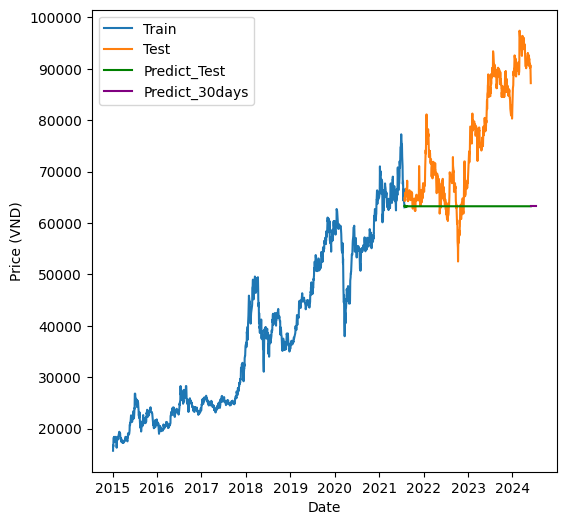
\includegraphics[width=\linewidth]{bibliography/RNN/VCB(7-3).png}
    \caption{RNN model's result with 7:3 splitting proportion}
    \label{fig8}
  \end{minipage}
\end{figure}

\begin{figure}[H]
  \centering
  \begin{minipage}{0.7\linewidth}
    \centering
    \includegraphics[width=\linewidth]{bibliography/GRU/VCB(9-1).png}
    \caption{GRU model's result with 9:1 splitting proportion}
    \label{fig8}
  \end{minipage}
\end{figure}

\begin{figure}[H]
  \centering
  \begin{minipage}{0.7\linewidth}
    \centering
    \includegraphics[width=\linewidth]{bibliography/LSTM/VCB(9-1).png}
    \caption{LSTM model's result with 9:1 splitting proportion}
    \label{fig8}
  \end{minipage}
\end{figure}

\begin{figure}[H]
  \centering
  \begin{minipage}{0.7\linewidth}
    \centering
    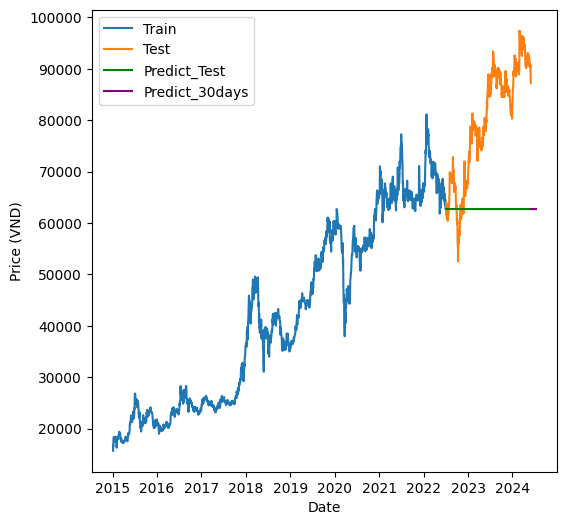
\includegraphics[width=\linewidth]{bibliography/MLP/VCB(8-2).png}
    \caption{MLP model's result with 8:2 splitting proportion}
    \label{fig8}
  \end{minipage}
\end{figure}

\subsection{BID dataset} 
\begin{table}[H]
    \centering
    \renewcommand{\arraystretch}{1.1}
    \begin{tabular}{|c|c|c|c|c|}
         \hline
         \multicolumn{5}{|c|}{\textbf{BID Dataset's Evaluation}}\\
         \hline
         \centering Model & Train:Test & RMSE & MAPE (\%) & MAE\\
         \hline
         \multirow{3}{*}{LinearRegression} 
         & 7:3 & 822.182 & 1.597 & 594.782 \\ 
         & \textbf{8:2} & \textbf{820.474} & \textbf{1.485} & \textbf{593.121} \\ 
         & 9:1 & 834.095 & 1.354 & 612.316\\
         \hline
         \multirow{3}{*}{ARIMA} 
         & 7:3 & 10079.951 & 19.105 & 7954.857\\ 
         & 8:2 & 9970.061 & 19.103 & 8243.155 \\ 
         & \textbf{9:1} & \textbf{7728.882} & \textbf{12.459} & \textbf{5975.497}\\
         \hline
         \multirow{3}{*}{RNN} 
         & 7:3 & 1053.944 & 1.979 & 774.755 \\ 
         & 8:2 & 827.201 & 1.54 & 601.537 \\ 
         & \textbf{9:1} & \textbf{936.1}  & \textbf{1.507} & \textbf{683.849}\\
         \hline
         \multirow{3}{*}{GRU} 
         & 7:3 &  922.985 &  1.782 & 683.561 \\ 
         & 8:2 &  881.985 & 1.574 & 637.272 \\ 
         & \textbf{9:1} & \textbf{819.893}  & \textbf{1.388} & \textbf{620.413}\\
         \hline
         \multirow{3}{*}{LSTM} 
         & \textbf{7:3} & \textbf{954.939} & \textbf{1.839} & \textbf{706.562} \\ 
         & 8:2 & 1098.96 & 2.01 & 842.664 \\ 
         & 9:1 & 1243.067  & 2.035 & 963.498\\
         \hline
         \multirow{3}{*}{MLP} 
         & 7:3 & 1220.597 & 2.682 & 995.578 \\ 
         & \textbf{8:2} & \textbf{896.795} & \textbf{1.636} & \textbf{655.182} \\ 
         & 9:1 & 982.078 & 1.548 & 715.512\\
         \hline
         \multirow{3}{*}{MLP + Nadam} 
         & 7:3 & 1018,737 & 1,963 & 752,029 \\ 
         & \textbf{8:2} & \textbf{907,84} &\textbf{1,677} & \textbf{670,579} \\ 
         & 9:1 & 1925,255 & 3,826 & 1747,529 \\
         \hline
         \multirow{3}{*}{MLP + Adadelta} 
         & 7:3 & 3330.254 &  6.812 &  2620.923 \\ 
         & \textbf{8:2} & \textbf{1324.327} &  \textbf{2.595} &  \textbf{1034.115} \\ 
         & 9:1 & 1809.620 & 3.202 & 1442.423\\
         \hline
    \end{tabular}
    \caption{BID Dataset's Evaluation}
    \label{vcbresult}
\end{table}

\begin{figure}[H]
  \centering
  \begin{minipage}{0.7\linewidth}
    \centering
    \includegraphics[width=\linewidth]{bibliography/RNN/BID(9-1).png}
    \caption{RNN model's result with 9:1 splitting proportion}
    \label{fig8}
  \end{minipage}
\end{figure}

\begin{figure}[H]
  \centering
  \begin{minipage}{0.7\linewidth}
    \centering
    \includegraphics[width=\linewidth]{bibliography/GRU/BID(9-1).png}
    \caption{GRU model's result with 9:1 splitting proportion}
    \label{fig8}
  \end{minipage}
\end{figure}

\begin{figure}[H]
  \centering
  \begin{minipage}{0.7\linewidth}
    \centering
    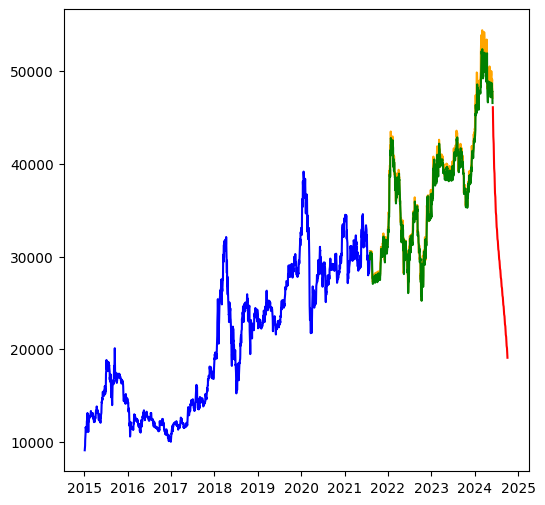
\includegraphics[width=\linewidth]{bibliography/LSTM/BID(7-3).png}
    \caption{LSTM model's result with 7:3 splitting proportion}
    \label{fig8}
  \end{minipage}
\end{figure}

\begin{figure}[H]
  \centering
  \begin{minipage}{0.7\linewidth}
    \centering
    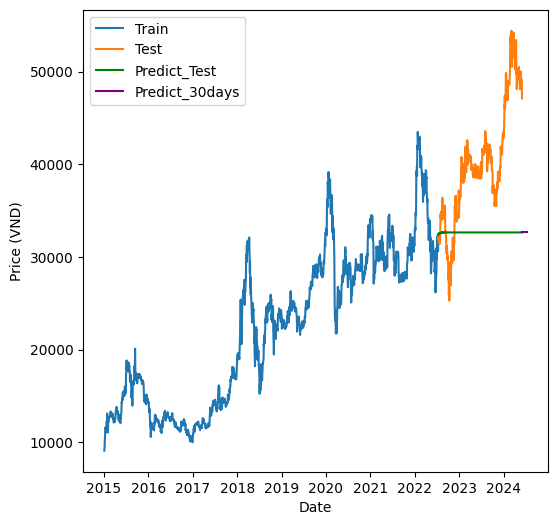
\includegraphics[width=\linewidth]{bibliography/MLP/BID(8-2).png}
    \caption{MLP model's result with 8:2 splitting proportion}
    \label{fig8}
  \end{minipage}
\end{figure}


\subsection{CTG dataset}
\begin{table}[H]
    \centering
    \renewcommand{\arraystretch}{1.1}
    \begin{tabular}{|c|c|c|c|c|}
         \hline
         \multicolumn{5}{|c|}{\textbf{CTG Dataset's Evaluation}}\\
         \hline
         \centering Model & Train:Test & RMSE & MAPE (\%) & MAE\\
         \hline
         \multirow{3}{*}{LinearRegression} 
         & 7:3 & 582.08 & 1.614 & 425.579 \\ 
         & \textbf{8:2} & \textbf{548.029} & \textbf{1.466} & \textbf{394.24} \\ 
         & 9:1 & 578.528 & 1.328 & 410.543\\
         \hline
         \multirow{3}{*}{ARIMA} 
         & 7:3 & 4599.286 & 15.521 & 3915.266\\ 
         & 8:2 & 5601.481 & 15.535 & 4502.582 \\ 
         & \textbf{9:1} & \textbf{4935.34} & \textbf{11.122} & \textbf{3623.256}\\
         \hline
         \multirow{3}{*}{RNN} 
         & 7:3 & 823.732 & 2.539 & 678.896 \\ 
         & 8:2 & 1227.0 & 4.183 & 1119.526 \\ 
         & \textbf{9:1} & \textbf{634.317}  & \textbf{1.633} & \textbf{484.374}\\
         \hline
         \multirow{3}{*}{GRU} 
         & 7:3 &  575.480 &  1.595 & 423.656 \\ 
         & \textbf{8:2} &  \textbf{545.471} & \textbf{1.451} & \textbf{389.686} \\ 
         & 9:1 & 575.852  & 1.349 & 414.24\\
         \hline
         \multirow{3}{*}{LSTM} 
         & \textbf{7:3} & \textbf{593.119} & \textbf{1.678} & \textbf{442.965} \\ 
         & 8:2 & 662.685 & 1.857 & 510.267 \\ 
         & 9:1 & 669.614 & 1.586 & 492.945\\
         \hline
         \multirow{3}{*}{MLP} 
         & \textbf{7:3} & \textbf{623.118} & \textbf{1.758} & \textbf{465.702} \\ 
         & 8:2 &	815.214 & 2.389 & 650.622 \\ 
         & 9:1 & 1666.636 & 1.576 & 1405.051\\
         \hline
         \multirow{3}{*}{MLP + Nadam} 
         & 7:3 & 740,389 & 2,197 & 582,564 \\ 
         & \textbf{8:2} & \textbf{591,791} & \textbf{1,62} & \textbf{437,889} \\ 
         & 9:1 & 1225,713 & 3,435 & 1064,49 \\
         \hline
         \multirow{3}{*}{MLP + Adadelta} 
         & 7:3 & 1765.624 &  5.097 &  1340.111 \\ 
         & \textbf{8:2} & \textbf{1356.085} & \textbf{3.754} &  \textbf{1025.133} \\ 
         & 9:1 & 2858.715 & 2.725 & 2436.841\\
         \hline
    \end{tabular}
    \caption{CTG Dataset's Evaluation}
    \label{vcbresult}
\end{table}

\begin{figure}[H]
  \centering
  \begin{minipage}{0.7\linewidth}
    \centering
    \includegraphics[width=\linewidth]{bibliography/RNN/CTG(9-1).png}
    \caption{RNN model's result with 9:1 splitting proportion}
    \label{fig8}
  \end{minipage}
\end{figure}

\begin{figure}[H]
  \centering
  \begin{minipage}{0.7\linewidth}
    \centering
    \includegraphics[width=\linewidth]{bibliography/GRU/CTG(9-1).png}
    \caption{GRU model's result with 8:2 splitting proportion}
    \label{fig8}
  \end{minipage}
\end{figure}

\begin{figure}[H]
  \centering
  \begin{minipage}{0.7\linewidth}
    \centering
    \includegraphics[width=\linewidth]{bibliography/LSTM/CTG(7-3).png}
    \caption{LSTM model's result with 7:3 splitting proportion}
    \label{fig8}
  \end{minipage}
\end{figure}

\begin{figure}[H]
  \centering
  \begin{minipage}{0.7\linewidth}
    \centering
    \includegraphics[width=\linewidth]{bibliography/MLP/CTG(7-3).png}
    \caption{MLP model's result with 7:3 splitting proportion}
    \label{fig8}
  \end{minipage}
\end{figure}

\section{Conclusion}
After employing six algorithms: ARIMA, Linear Regression, RNN, LSTM, GRU, MLP on three different datasets about stock prices BID, CTG and VCB, we found that the model GRU and LSTM are the two best algorithms giving the best results based on three measures RMSE, MAPE, MAE on all six algorithms. Moreover, between Nadam and Adadelta, Nadam always gives better results and better at minimizing loss function. 
\subsection{Summary}
In the realm of stock price forecasting, a wide range of methodologies has been explored, spanning from traditional statistical models to cutting-edge machine learning algorithms. Among the performed models, Linear Reregression (LR), Auto Regressive Integrated Moving Average (ARIMA), GRU, LSTM,RNN and MLP, it shows evident thatGRU and LSTM as the most promising and effective models for predicting stock prices. While Nadam optimization is better than Adadelta optimization in terms of better results.\\ Evaluation metrics such as RMSE, MAPE, and MSLE consistently highlight the superior performance of the  GRU, and LSTM models across various aspects of forecasting accuracy. Their ability to handle the inherent uncertainties of stock markets makes them powerful tools for investors and analysts seeking reliable predictions.
\subsection{Future Considerations}
In our future research, we want to try other optimization algorithms with different deep learning models:\\
\indent\textbullet\ Enhancing the accuracy of the model. While the above algorithms have demonstrated promising results in predicting stock prices, there are some methods that improve the accuracy to ensure more precise forecasting outcomes.\\
\indent\textbullet\ Exploring alternative deep learning algorithms. Ensemble techniques, such as combining multiple models or using various ensemble learning methods, can also improve the robustness and accuracy of the forecasts.\\
\indent\textbullet\ Researching new forecasting models. The field of forecasting continuously evolves, with new algorithms and models being researched and developed.\\
By continuously exploring and incorporating new features, data sources, and modeling techniques, we can strive for ongoing optimization of the forecasting models and enhance their ability to predict stock prices with greater precision and reliability.
\section*{Acknowledgment}
\addcontentsline{toc}{section}{Acknowledgment}
First and foremost, we would like to express our sincere gratitude to \textbf{Assoc. Prof. Dr. Nguyen Dinh Thuan} and \textbf{Mr. Nguyen Minh Nhut} for their exceptional guidance, expertise, and invaluable feedback throughout the research process. Their mentorship and unwavering support have been instrumental in shaping the direction and quality of this study. Their profound knowledge, critical insights, and attention to detail have significantly contributed to the success of this research.
\\This research would not have been possible without the support and contributions of our mentors. We would like to extend our heartfelt thanks to everyone involved for their invaluable assistance, encouragement, and belief in our research. Thank you all for your invaluable assistance and encouragement.

%% UNCOMMENT these lines below (and remove the 2 commands above) if you want to embed the bibliografy.
\begin{thebibliography}{00}
\bibitem{b1} 
    Somenath Mukherjee, 
    Bikash Sadhukhan,
    Stock market prediction using deep learning algorithms,
    ResearchGate,   \url{https://www.researchgate.net/publication/354268488_Stock_market_prediction_using_deep_learning_algorithms}
    
\bibitem{b2} 
    Shahzad Zaheer, 
    Nadeem Anjum,
    Saddam Hussain, 
    Abeer D. Algarni, 
    Jawaid Iqbal, 
    Sami Bourouis,
    Syed Sajid Ullah,
    A Multi Parameter Forecasting for Stock Time Series Data Using LSTM and Deep Learning Model,
    \url{https://www.mdpi.com/2227-7390/11/3/590}

\bibitem{b3} 
    Nayab Minhaj, Roohi Ahmed, Irum Abdul Khalique, Mohammad Imran,
    A  Comparative  Research  of  Stock  Price  Prediction  of  Selected  Stock  Indexes and the Stock Market by Using Arima Model, \url{https://ojs.wiserpub.com/index.php/GES/article/view/1426/1046}

\bibitem{b4} 
    Jatin Sharma1,
    Sameer Soni,
    Priyanka Paliwal,
    Shaik Saboor,
    Prem K. Chaurasiya,
    Mohsen Sharifpur,
    Nima Khalilpoor,
    Asif Afzal,
    A novel long term solar photovoltaic power forecastingapproach using LSTM with Nadam optimizer: A case studyof India,
    \url{https://onlinelibrary.wiley.com/doi/epdf/10.1002/ese3.1178}

\bibitem{b5} 
    Matthew D. Zeiler,
    ADADELTA: AN ADAPTIVE LEARNING RATE METHOD, 
    \url{https://browse.arxiv.org/pdf/1212.5701v1}

\bibitem{b6}
    Vivek Kumar Prasad,
    Stock Market Prediction with Deep Learning: A Case Study on MLP and LSTM. Journal of Financial Technology and Data Science,
    \url{https://link.springer.com/chapter/10.1007/978-981-99-1479-1_35}
    
\bibitem{b7} 
    Rebecca Bevans,
    Multiple Linear Regression, 
    Published on February 20,2020,\url{https://www.scribbr.com/statistics/multiple-linear-regression/}

\bibitem{b8} 
    Duke University,
    ARIMA models for time series forecasting, 
    \url{https://people.duke.edu/~rnau/411arim.htm}

\bibitem{b9} 
    FARHAD MORTEZAPOUR SHIRI,
    A Comprehensive Overview and Comparative Analysis on Deep 
Learning Models: CNN, RNN, LSTM, GRU, 
    \url{https://arxiv.org/pdf/2305.17473}

\bibitem{b10} 
    Zachary C. Lipton,
    A Critical Review of Recurrent Neural Networks for Sequence Learning, \url{https://arxiv.org/abs/1506.00019}
    
\bibitem{b11} 
    Rishikesh Gawde,
    Image Caption Generation Methodologies, \url{https://www.researchgate.net/publication/351840108_Image_Caption_Generation_Methodologies}
    
\bibitem{b12} 
    Savvas Varsamopoulos,
    Designing neural network based decoders for surface codes, \url{https://www.researchgate.net/publication/329362532_Designing_neural_network_based_decoders_for_surface_codes}

\bibitem{b13} 
    Savvas Varsamopoulos,
    Forecasting stock prices with long-short term memory neural network based on attention mechanism,
    \url{https://journals.plos.org/plosone/article?id=10.1371/journal.pone.0227222}

\bibitem{b14} 
    Iqbal H. Sarker,
    Deep Learning: A Comprehensive Overview on Techniques, Taxonomy, Applications and Research Directions,
    \url{https://link.springer.com/article/10.1007/s42979-021-00815-1}

\bibitem{b15} 
    Kun-Cheng Ke,
    Quality Prediction for Injection Molding by Using a Multilayer Perceptron Neural Network,
    \url{https://link.springer.com/article/10.1007/s42979-021-00815-1}

\bibitem{b16} 
    Shiksha Online,
    What is a multilayer perceptron (MLP) neural network?,
    \url{https://www.shiksha.com/online-courses/articles/understanding-multilayer-perceptron-mlp-neural-networks/}

\end{thebibliography}
%%%%%%%%%%%%%%%

\EOD

\end{document}
